\section{Introduction}
The presence of sensors in the ubiquitous environment has led to the production of an enormous amount of data. These sensors belong to diverse categories including planar pressure, thermal, optical, acoustic, and proximity modalities. 
They provide information for activity recognition and context-aware models that could be used for a wide range of applications such as automatic monitoring in the smart environment and wellness scene, computer-human-interaction, user experience, etc. 
%The information and feedback provided by the sensors are used to get the context in which they are placed and extract useful information to solve a purpose, mainly to benefit humans. 
There has been extensive research on wearable and pervasive sensors, which record and sense data in the context of human activities; ranging from physical activities (running, sleeping, walking, etc.), such as  monitoring gym exercises \cite{zhou2016never}, analyzing gait patterns \cite{tao2012gait}, to biological activities (breathing, eating, etc.), such as breathing detection \cite{corbishley2008breathing}, eating \cite{cheng2010active} and drinking arm gesture detection \cite{amft2005detection}. The task of extracting useful information from the raw sensor data has been performed using various machine learning and data mining techniques \cite{banaee2013data}. One of the many examples is the use of such methods in human activity recognition \cite{maurer2006activity}. Usually, when the raw sensor data is concerned, the feature extraction is done using numerical statistical features. These features have proven to be quite reliable in tasks related to classification, recognition and segmentation \cite{cheng2013smart}. 
\par

Deep learning has been recently proven to be extremely successful in various domains. Convolutional neural networks (CNNs) \cite{fukushima1979neural}, have already been applied to practical tasks by Le Cun et al. \cite{le1990handwritten}, they have recently risen in popularity after achieving superhuman accuracy on image classification tasks \cite{krizhevsky2012imagenet,he2015deep,zhang2016polynet,szegedy2016inception}. Recurrent neural networks (RNN) especially with Long Short-Term Memory cells (LSTM) \cite{hochreiter1997long} have been used to classify sequences \cite{graves2008unconstrained} and to recognize activities \cite{donahue2015long, du2015hierarchical} with varying degrees of success. Both, CNN and RNN have been used in combination to create systems which are capable of understanding images, and to provide temporal context to these individual images. 

\par

A limitation of these techniques, however, is the requirement of large amounts of labeled data to facilitate the training of these very deep networks. While the computer vision community has facilitated this requirement with large labeled datasets, such as, the ImageNet \cite{ILSVRC15} and MS-COCO \cite{lin2014microsoft} datasets for object recognition, classification, detection and captioning; for various other tasks not many labeled datasets exist because the scope can be very specific when compared to general images.

\subsection{Transfer Learning}
For many Computer Vision problems, the above-mentioned limitation can be bypassed by performing transfer learning, i.e., using labeled data from one domain and transferring the learned knowledge to a target domain. Transfer learning involves using the knowledge acquired on a specific task, and adapting this knowledge to a different, but related task. Caruana \cite{caruana1998multitask} first introduced the concept of multi-task learning, targeting the improvement in generalization by using the domain information of related tasks. A common scenario for transfer learning involves using a convolutional neural network trained on a very large dataset, and then further fine-tuning it on the target dataset which is relatively small in size. A pre-trained CNN is used for transfer learning by removing the last fully-connected layer and using the activations of the last hidden layer as the feature descriptors of the input dataset. The resulting feature descriptors are then used to train a classification model. Recently, transfer learning has been done on semantic segmentation of images  \cite{long2015fully}. The learned representations of fully convolutional networks like AlexNet \cite{krizhevsky2012imagenet}, VGGnet \cite{vgg} are transferred by fine-tuning the semantic segmentation task. Similarly, Li et al. explored the concept of transfer learning on images with limited semantic meanings which do not perform well for high level visual tasks. The use of large number of pre-trained generic object detectors improved performances on recognition tasks with simple classifiers like linear SVM \cite{li2010object}. The key advantage of transfer learning is that it removes the need to create a large dataset required to train the CNNs. Also, the time and computational resources needed to perform training on such a large scale is considerably high and thus, transfer learning benefits us by saving this additional cost.

\par
Conventionally, transfer learning has been performed on domains that are easily visually interpretable. We define a domain as being easily visually interpretable as follows:
\\\\
\emph{A domain is said to be easily visually interpretable if by looking at its visual representation, a human can extract relevant information and a sense of the meaning it conveys.}
\\\\
Additionally, if the data is conventionally visually interpreted, it belongs to the category of easily visually interpretable data. For example, images of everyday objects such as automobiles, animals, landscapes; documents, X-ray, and MRI scan data all belong to the category of easily visually interpretable images. In the context of these examples, an average human can easily learn to distinguish between different classes, e.g., several sub-species of animals (Fig. \ref{fig:imagenet}(c)(d)) or several models of automobiles \cite{russakovsky2015imagenet}. Also the classification of documents into categories such as legal, scientific, or historical is a trivial task for most people. Doctors or radiologists analyze and interpret MRI or X-ray data (See Fig. \ref{fig:imagenet}(a)(b)) to detect irregularities in healthy organs. The application of transfer learning on such images is feasible for mainly two reasons. Firstly, it is possible due to their nature of being visually meaningful and secondly, there are large datasets from the same domain available within the community to carry out the transfer learning tasks. 

However, there exist types of data, such as sensor data, which are not easily visually interpretable, and it is unclear if it would be possible to visually interpret them. Not visually interpretable data can be, for example, position updates of moving objects in location-based services, fluctuations in the stock market, medical experimental observations, or streaming sensor data.  An example is illustrated in Fig. \ref{fig:similar_steps} which shows the pressure mappings for a particular moment of a foot step. We can see that Fig. \ref{fig:similar_steps} (a) and (c) look similar but they belong to different persons. Similarly, Fig. \ref{fig:similar_steps} (a) and (b) look different but they belong to the same person. Hence, such sensor data is clearly not easily visually interpretable.

\begin{figure}
	\centering
	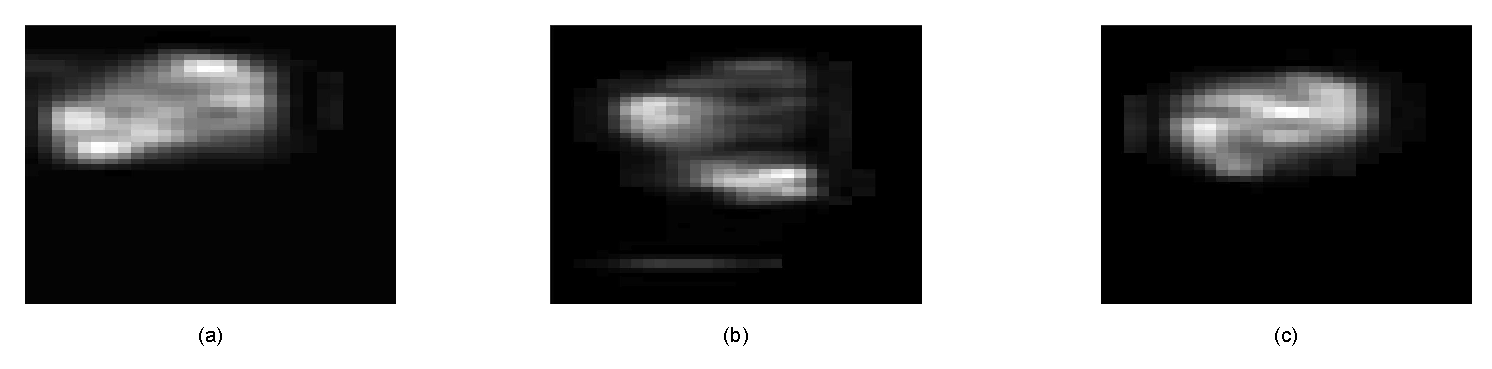
\includegraphics[width=8cm]{./figures/similar_steps.pdf}
	\caption{The transformed pressure sensor data corresponding to different moment of a step at different time. The heat maps (a) and (b) belong to the same person, (c) belongs to a different person.}
	\label{fig:similar_steps}
\end{figure}


% Paper Contribution
\subsection{Paper Contribution}
  In this paper, we introduce the idea of using the concept of transfer learning on a domain which is not easily visually interpretable. We carry out a shift procedure, which involves the shift from a domain which is not suitable for transfer learning to a domain on which the CNNs have been trained. This shift facilitates the use of transfer learning even for data which normally is not an ideal candidate for transfer learning. In order to show that such transformation is useful,  we extend the transfer learning methods on pressure sensor data. The raw sensor data is first transformed into a set of visual images and then used as an input dataset for a pre-trained convolutional network model. Thus, the core contributions of this paper are as follows:
\begin{itemize}
\item \textit{Modality transformation:} We transform non-interpretable data to the image domain and explore the effectiveness of deep neural networks. We observe that models which are pre-trained on the aesthetic and visually interpretable datasets like ImageNet, are powerful and accurate enough in terms of feature calculation that the artificially generated images are also recognized with high accuracy rates.

\item \textit{Unified feature extraction process:} Typically, the feature extraction process using conventional methods is customized for each unique application. In the case of sensor data, even with the same kind of sensors used for collecting the information, the feature extraction and data mining techniques vary depending on the target application of the data. The same pressure sensor has been used to cater to different applications \cite{cheng2016smart, SmartMat} but uses different feature extraction techniques. We provide a unified feature extraction process, which can be applied to the sensor data after conversion into the visual domain independent from its application.

\item \textit{Evaluation on pressure sensor data:} We evaluate our approach of modality transformation with pressure values of single steps as each person walks on a Smart-Mat \cite{SmartMat}, a fabric based real-time pressure force mapping system. The domain shift is carried out by transforming the pixel data values corresponding to the pressure exerted on the floor while walking (See Section \ref{pressuredata}), to the respective images. This information consisting of images serve as the input to pre-trained CNNs. With the application of our approach of modality transformation, we achieve a person identification accuracy of 87.66\% which significantly outperforms the state of the art (76.9 \%) (See Section \ref{sec:eval})

\end{itemize}

